\documentclass{tufte-handout}

\usepackage{../CommonLatexPackages/fall2018_preamble_v1.0}
\fancypagestyle{firstpage}

\def \BoD {Bridge of Doom\texttrademark}

{\rhead{Night 3 \linebreak \textit{Version: \today}}}

\title{Night 3: Crossing the Bridge of Doom}
\author{Quantitative Engineering Analysis}
\date{Spring 2019}

\begin{document}

\maketitle
\thispagestyle{firstpage}

\section{Overview}
Welcome to Robo Ninja Warrior.  Your first challenge, should you choose to accept it (and you should!), will be crossing the \emph{\BoD}.  This challenge will push you and your robot literally to the brink, requiring you to be at the height of your analytical powers.  Along the way you'll be building your knowledge of parametric curves, deriving robot motion models, and learning powerful validation and debugging techniques.
\begin{figure}
\begin{center}
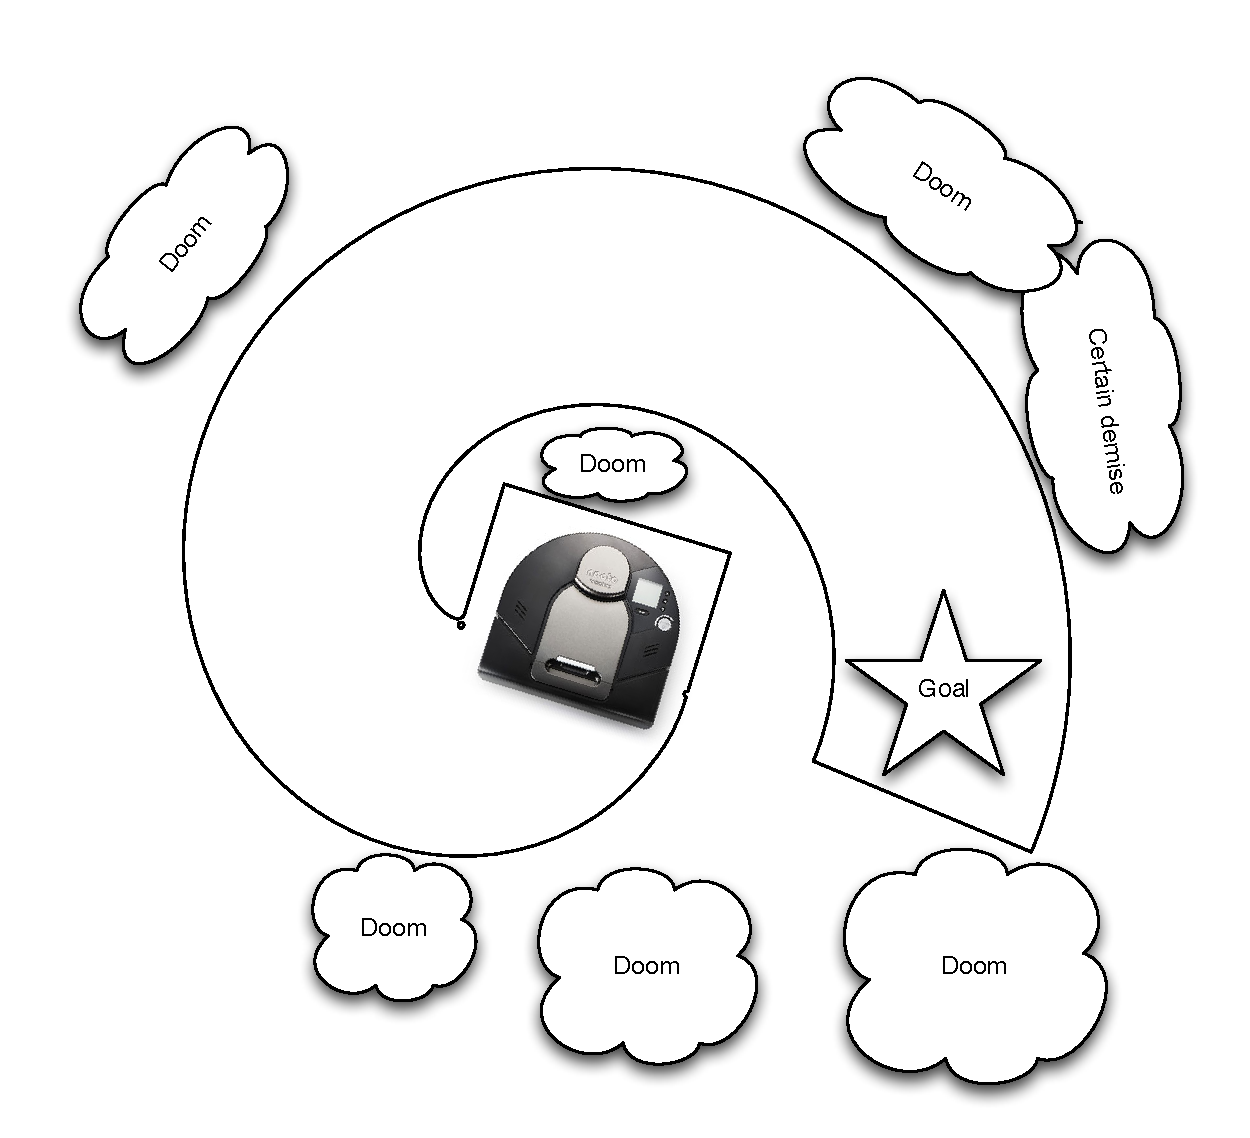
\includegraphics[width=8cm]{figures/bridge_sketch}
\end{center}
\caption{The \BoD. \label{fig:bridge_sketch}}
\end{figure}

\subsection{Learning Goals}

By the end of this challenge, you should be comfortable with the following:
\begin{enumerate}
\item Computing tangent vectors and normal vectors to parametric curves, and connecting these vectors to motion.
\item Deriving a motion model of a robot.
\item Validating a motion model of a robot empirically.
\item Controlling a robot using an open-loop control strategy.
\item Mapping the path of a robot based on encoder values.
\item Evaluating the performance of your robot based on an appropriate error metric.
\end{enumerate}

\section{The Challenge}
You will write a program to autonomously pilot your robot from the starting platform to the goal.  What lies between?  Ahh, that is the harrowing \BoD.  The shape of the centerline of the \BoD~is defined by one of the following parametric curves

\[\mathbf{r}(u) =  -2a\left(\left(l - \cos u \right) \cos u +\left(1 - l\right)\right) \hat{\mathbf{i}} + 2a (l - \cos u) \sin u \hat{\mathbf{j}} \; (u \in [0,2\pi], a = 0.4, l = 0.4). \]

or

\[\mathbf{r}(u) =  0.3960 \cos(2.65(u+1.4)) \mathbf{i} - 0.99 \sin(u+1.4) \mathbf{j}. \; (u \in [0,3.2]) \]

\section{(Re)Meet your Neato}

You've already achieved passing familiarity with your Neato (see Figure~\ref{fig:neato}), however, in this challenge you two will really get acquainted!  The Neato moves via differential drive, which we worked with in class Monday.  In this challenge you are tasked with piloting your robot across the \BoD.  In order to control your robot, you will be using open-loop control.  Open-loop control means that you will determine a sequence of motor commands (e.g., the velocities for each of the Neato's wheels) ahead of time.  You will then write a program that sends these motor commands to the robot at the prescribed times irrespective of where the robot is along the path.  Despite its simplicity, open-loop control can be quite powerful, and it is up to the task of crossing the \BoD.  That being said, if you are looking for ways to take this challenge to the next level, you can use sensor feedback to modify your path midstream.

\newthought{The maximum speed of your NEATO is roughly 0.3 meters per second.}

\begin{marginfigure}
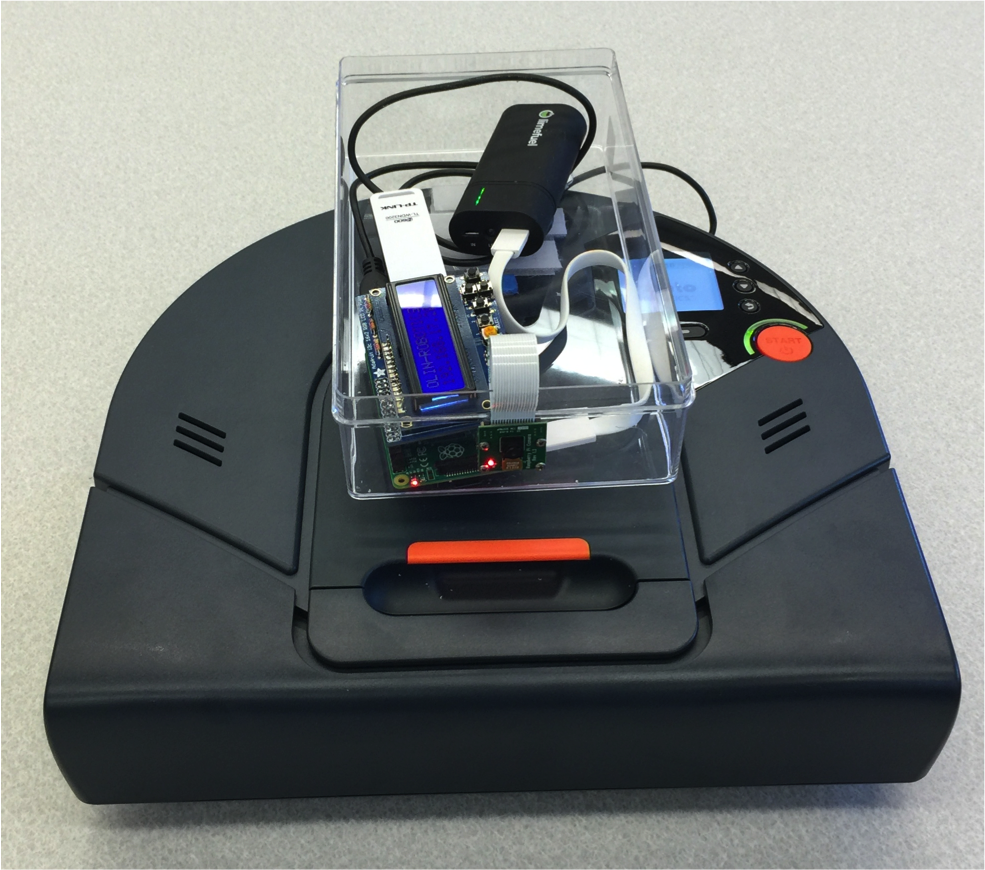
\includegraphics[width=6cm]{figures/neato.png}
\caption{The Neato in all its glory. The Neato will be your bot for the duration of this module.\label{fig:neato}}
\end{marginfigure}

\section{Crossing the Bridge of Doom}
Let's reflect on how far we've come towards completing our challenge.  We have developed equations for $V_L$ and $V_R$ that achieve a desired linear and angular velocity, and we have validated this model empirically.  All that remains is to program our robot to follow a parametric curve.

\begin{enumerate}[series=Deliverable, label=\textbf{Deliverable} (\arabic*)]

\item For the \BoD of your choosing, plot the parametric curve that defines the centerline of the bridge. On the same figure, plot the unit tangent and unit normal vectors at several points along the curve. You should have starter code to help with this in the Night 1 assignment.

\item Compute and plot your robot's left and right wheel velocities as a function of time for your chosen \BoD. After successfully traversing the bridge, add the measured wheel velocities to your plot. The planned (theoretical) velocities should be plotted with a solid line, while the experimental result should be plotted with a dashed line. Make sure your plots include appropriate units, labels, and legends.

\item Compute and plot your robot's planned linear speed and angular velocity as a function of time for the \BoD. After successfully traversing the bridge, add the measured linear speed and angular velocity to your plot. The planned (theoretical) speed and angular velocity should be plotted with a solid line, while the experimental result should be plotted with a dashed line. Make sure your plots include appropriate units, labels, and legends.

\item Write a program to send the appropriate control signal based on the time elapsed since the start of the path.  Be careful about handling the case when $|\r'(t)| = 0$.  In this case $\Nhat(t)$ is not defined and $\omega(t) = 0$.  Note, that you can always slow down or speed up your robot by multiplying $t$ by a constant (we have used the constant $\alpha$ in previous assignments for this purpose). Be careful since the maximum speed of each of the robot's wheels is $0.3 m / s$. Test your program thoroughly on the \BoD~while it is lying on the floor.  When you are convinced your system is working properly, add some danger.  Remember, always use a robot spotter when crossing the \BoD. Take a video of your robot crossing the \BoD.

\begin{marginfigure}
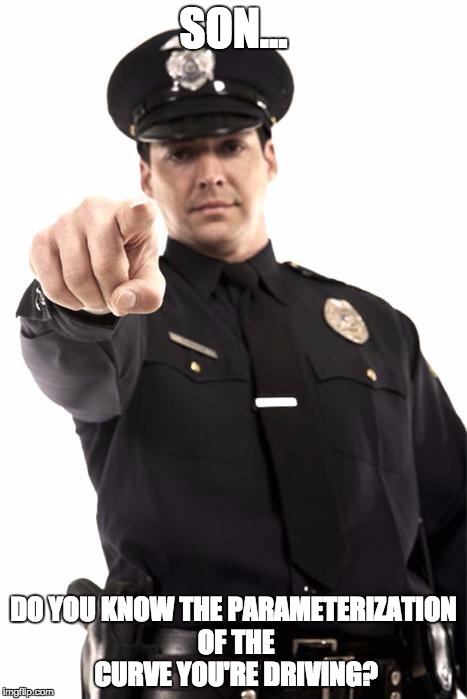
\includegraphics[width=\linewidth]{Figures/1m8rss.jpg}
\end{marginfigure}


\item Consider going to spectate the Boston Marathon. It is the best day of the year in the city. By far. (This is Jeff, BTW.) If you go, take a picture and include it in your writeup. Bonus points for making a sign that says ``Give me a high five so my Professor gives me bonus points''... and actually getting high fives for it. 

\item Map your robot's predicted and actual path crossing the \BoD by using the provided code to collect the wheel encoder data and convert that to coordinates and headings for the robot throughout its perilous journey.  Use the Matlab quiver command to plot the predicted and experimental unit tangent vectors at various points along the curve (note: do not include an arrow for every time step or your plot will be too cluttered). The planned (theoretical) path should be plotted with a solid line, while the experimental result should be plotted with a dashed line. Make sure your plots include appropriate units, labels, and legends.

\item Choose an appropriate error metric to compare your theoretical and experimental paths. Include an appropriate plot for your chosen metric (e.g. accumulated total error versus time, lateral distance from centerline versus distance traveled, etc.).

\begin{marginfigure}
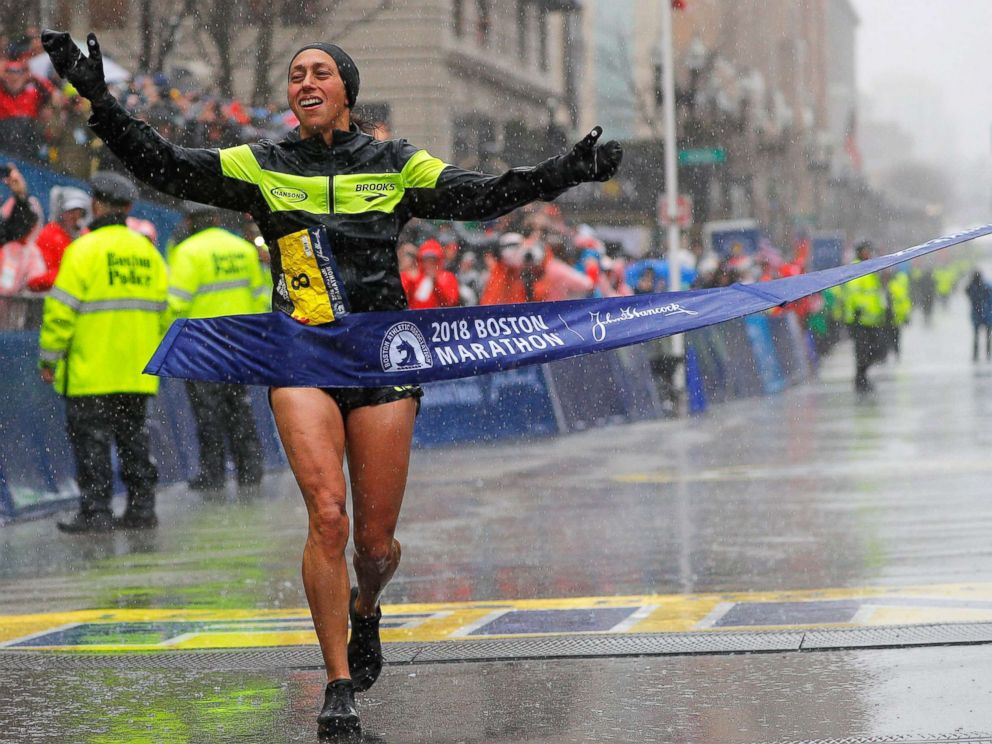
\includegraphics[width=5cm]{figures/linden2.jpg}
\caption{\emph{Some days it just flows and I feel like I'm born to do this, other days it feels like I'm trudging through hell. Every day I make the choice to show up and see what I've got, and to try and be better. My advice: keep showing up.}- 2018 Boston Marathon Champion Des Linden, first American woman to win in 33 years.}
\end{marginfigure}

\end{enumerate}

\section{Writing up Your Work}
Prepare a writeup of your work on this challenge.  Your writeup should contain the following components.
\begin{enumerate}
\item An introduction explaining the challenge and including the functional definition of the bridge you chose to cross.
\item A description of your general process including relevant equations.  What strategies did you try?  What worked?  What didn't?  We are looking for something relatively comprehensive.  A good length would be about a page of text. 
\item Each of the plots detailed above with appropriate captions. 
\item A discussion of your measured error and a justification of your chosen error metric.
\item A link to a youtube video of your robot in action (include a link in your writeup). Bonus points for high production value like \href{https://www.youtube.com/watch?v=9zWqHOggKSs}{this}.
\end{enumerate}

In addition to the writeup, you should also turn in your carefully commented code (you could add a link to a Github repo in your writeup, or upload your MATLAB code files to your Canvas submission).

\section{Optional Extensions}

\begin{enumerate}[series=extension, label=\textbf{Extension} (\arabic*)]
\item One weakness of the approach that you implemented is that it doesn't take into account the fact that the robot doesn't instantaneously do what you tell it to do.  One possible way to remedy this is to monitor the robot's position over time using live readings of the wheel encoders.  In class on Day 3 you derived a method for updating the robot's position and orientation given measurements of its wheel velocities.  We call this estimate of the robot's position its odometry.  By comparing the robot's position as determined by its odometry with the desired position (given by $\mathbf{r}(t)$) you can try to correct your robot's motion to more faithfully follow the path.  How you accomplish this exactly is up to your own creativity and analysis skills.

\item In Night 1 of the Boats module you proposed a set of mathematical curves that were a good approximation for the curves of a fruit or vegetable. Here is your opportunity to have a robot drive a fruit or vegetable shaped trajectory, and plot the resulting path using encoder data. Take a video if you do this!

\end{enumerate}

\end{document}
